\documentclass[letterpaper,12pt]{report}
\usepackage{fullpage}
\usepackage{amsmath, amsthm, amssymb}
\usepackage{graphicx}
\usepackage{verbatim}
\usepackage{fancyhdr}
\usepackage[colorlinks=true,linkcolor=blue]{hyperref}
\usepackage[all]{xy}

\newtheorem{definition}{Definition}[chapter]
\newtheorem{theorem}{Theorem}[chapter]
\theoremstyle{plain}
\newtheorem*{thmHop}{The hopping immunity theorem}
\theoremstyle{definition}
\newtheorem*{example}{Example}

\graphicspath{{Images/}}
 
\renewcommand\topfraction{.9}
\renewcommand\textfraction{.05}
\makeatletter
\begin{comment}
\renewcommand\chapter{\if@openright\cleardoublepage\else\clearpage\fi
                    \thispagestyle{fancy}%
                    \global\@topnum\z@
                    \@afterindentfalse
                    \secdef\@chapter\@schapter}
                    \end{comment}
\makeatother

\title{\textbf{Analysis of block survival probabilities}}

\author{Assaf Shomer\\
}

\date{\today}

\begin{document}

\maketitle
%\pagestyle{fancy}
\begin{abstract}
Analysis of block survival probabilities in the presence of miners that employ non-traditional mining strategies in the interest of increasing their reward
\end{abstract}
\pagenumbering{roman}
\tableofcontents
\chapter{Introduction}\label{chap:intro}
\pagenumbering{arabic}
\section{Bitcoin and mining}
Bitcoin is the world's first decentralized digital currency (\cite{Bitcoin}). blah blah
\section{The attack strategy}

\subsection{Honest Miners}
The honest miners following the bitcoin protocol described in \cite{Bitcoin}, publish each block as soon as it is discovered and switch their mining efforts to the head of the block-chain any time a new block is found. 
\subsection{Block withholding Miners}
The attackers do not share their newly found blocks and instead work on a $\bf{secret}$ branch of the block-tree until such time that their branch is longer than the main branch. At this time they can publish it and uproot the last $n$ (honestly mined) blocks in favour of their $m>n$ secretly mined ones.

\subsection{Goal}\label{subsec:goal}

Our goal is to calculate the probability that an honestly mined block is retained in the block-chain in the face of an attacker of relative power $q$. We will calculate this quantity by calculating the complement probability that a block withholding attacker succeeds in decapitating the block-chain mined on top of a given block.

\section{Setup}\label{calcsetup}
Let us denote by $\mathcal{H}$ the total hashing power of the network and divide it abstractly into an \emph{Honest} part which holds a portion $p\mathcal{H}$ of the total hashing power (where $p \in [0,1]$) and an \emph{Attacker} which holds the rest $q\mathcal{H}=(1-p)\mathcal{H}$. 

We start our analysis at a given point in time where the block-chain is of length $L$ and denote the last block mined as $\mathit{B}_L$. As time marches on the honest miners continue to mine on top of it ( $\mathit{B}_{L+1}, \mathit{B}_{L+2}, \dots$) while the attackers are building a separate branch on top of $\mathit{B}_L$ ( $\mathit{\tilde{B}}_{L+1}, \mathit{\tilde{B}}_{L+2}, \dots$) with the hope of overtaking it.

Treating block mining as a negative binomial random variable, the probability $\mathit{P_{n,p}(m)}$ that $m$ blocks are mined by the attackers $\mathbf{before}$ $n$ blocks were honestly mined is proportional to $p^nq^m$ and can be shown
(appendix \ref{app:probmath}) to be given by

\begin{equation}\label{eq:pnm}
\mathit{P}_{n,p}(m)={n + m -1\choose m}p^nq^m \quad n=1,2,\dots
\end{equation}

The probability $\mathit{a}_{n,m}(p)$ that the attackers manage to overtake the block-chain given the situation above\footnote{Namely, that the honest network mined $n$ blocks on top of $\mathit{B}_L$ and the attackers managed, during that time, to mine $m$ blocks on top of $\mathit{B}_L$ constituting their hidden branch.} is given by a Markov chain that depends only on the advantage $z$ of the honest network over the attackers $z=n-m$ defined by the recurrence relation

\begin{equation}\label{eq:markov}
\mathit{a}_z(p)=p\mathit{a}_{z+1}(p)+q\mathit{a}_{z-1}(p)
\end{equation}

The relation can be solved with boundary conditions $\mathit{a}_{-1}=&1, \mathit{a}_{\infty}=&0$ by

\begin{equation}\label{eq:az}
\mathit{a}_z(p)=\begin{cases}\left( \dfrac{q}{p}\right)^{z+1} & q\in [0,\dfrac{1}{2}] \quad \mathrm{and} \quad z=0,1,2\dots \\ \quad 1 & \mathrm{otherwise} \end{cases}
\end{equation}

For example, to find the probability of a double spend after $n$ confirmations, the attacker needs to mine $B_{L+1}$ (assumed as the starting point so no need to multiply by $q$) and then catchup from a deficit of $n-(m+1)$ where the extra block is the block where the double spend occurs.
This was calculated in \cite{Doublespend} to be 
\begin{equation}
D_n(p)=\sum_{m=0}^{\infty}P_{n,p}(m)\mathit{a}_{n-(m+1)}(p)
\end{equation}

\section{Probability of success}

In this paper, as explained in \ref{subsec:goal}, we are interested in a different quantity.

Let $\mathit{Q}(p)$  be the probability that the attackers succeed in decapitating the block-chain on top of $\mathit{B}_L$. This event occurs if the attackers manage to catch-up on $B_{L+1}$ after starting with $m=0,1,\dots$ blocks\footnote{Note that we do not need to multiply this by the probability $p$ that the honest miners mine the next block. This fact is implicit in the probability distribution \ref{eq:pnm} calculated under the assumption that the $n^{th}$ block is mined by the honest miners.}.

Formally 

\begin{equation}\label{eq:rnpdef}
\mathit{Q}(p)=\sum_{m=0}^{\infty}\mathit{P}_{1,p}(m)\mathit{a}_{1-m}(p)
\end{equation}

which results to (see details in appendix \ref{app:calcqofp})

\begin{equation}\label{eq:qofp}
\mathit{Q}(p)=
\begin{cases}
\dfrac{q^2}{1-q}\left(
3-2q
\right) & \quad q \in [0,\dfrac{1}{2}] \\
1 & \quad q \in [\dfrac{1}{2},1] 
\end{cases}
\end{equation}


In Figure ~\ref{fig:PlotProbOfSuccess} we plot the probability of a successful attack as a function of the relative hashing power $q$ against the probability of the attacker being honest, in which case his probability of success is just $q$

\begin{figure}[pos]
\centering
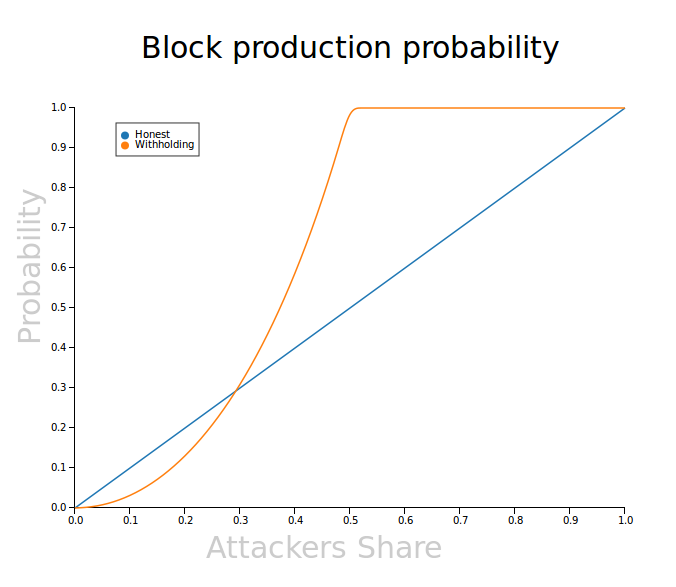
\includegraphics[width=150mm]{blocksurvival.png}
\caption{The orange curve plots the probability that the attackers manage to uproot the next honest block and replace it with one of their own. The blue curve is the baseline probability for an honest miner with the same hashing power $q$}
\label{fig:PlotProbOfSuccess}
\end{figure}

We see that an attacker improves his chances in the range $q>1-\dfrac{1}{\sqrt{2}} \sim 0.293$
\newpage
\section{Attacker's reward}
Next we calculate the expected reward of a block-withholding attacker.
We assume for simplicity that the reward of each party is simply proportional to the number of blocks mined by that party.

Formally

\begin{equation}\label{eq:rofpdef}
\mathit{R}(p)=\sum_{m=0}^{\infty}m\cdot\mathit{P}_{1,p}(m)\mathit{a}_{1-m}(p)
\end{equation}

which results to (see details in appendix \ref{app:calcrofp})

\begin{equation}\label{eq:rofp}
\mathit{R}(p)=
\begin{cases}
\dfrac{q^2}{1-q}\left(
3-2q
\right) & \quad q \in [0,\dfrac{1}{2}] \\
\dfrac{q}{1-q} & \quad q \in [\dfrac{1}{2},1] 
\end{cases}
\end{equation}


In Figure ~\ref{fig:AttackersReward} we plot the attackers reward as a function of the relative hashing power $q$ against the probability of the reward for an honest miner with the same hashing power, which is just $q$.

\begin{figure}[reward]
\centering
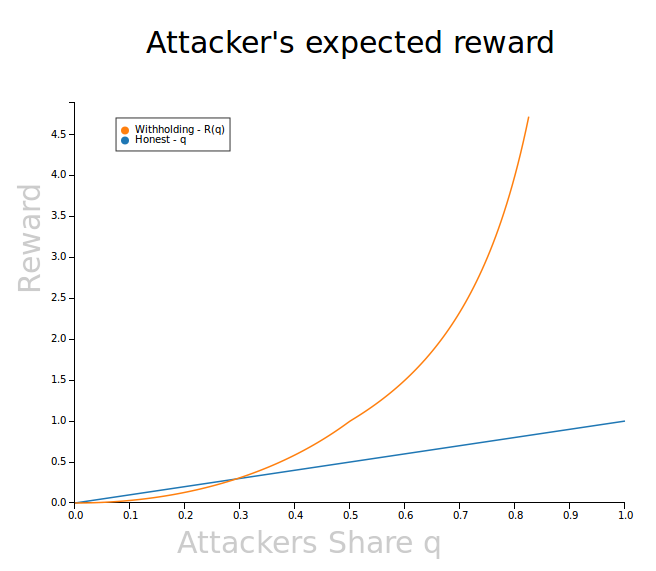
\includegraphics[width=150mm]{AttackersReward.png}
\caption{The orange curve plots the attacker's reward. The blue curve is the baseline reward for an honest miner with the same hashing power $q$.}
\label{fig:AttackersReward}
\end{figure}

We note a few things.
\begin{itemize}
\item In the range $q\in[0,\dfrac{1}{2}]$ $R(p)$ is identical to $Q(p)$.
  \item As expected the reward of the attackers exceeds the honest reward at the same point where the probability of success exceeds the honest benchmark. i.e. when $q>1-\dfrac{1}{\sqrt{2}} \sim 0.293$
  \item As $q\rightarrow 1$ the reward of the attackers diverges, because he basically controls the blockchain and can plant as many blocks as he desires.
  \item This may be a little hard to see in Figure ~\ref{fig:AttackersReward} but The function $R(p)$ is continuous but not continuously differentiable. At the point $q=\dfrac{1}{2}$ the derivative jumps from $4$ to $5$ (see appendix \ref{app:derivative} for details).
\end{itemize}





\appendix
\chapter{Calculation Details}
\section{Probability distribution} \label{app:probmath}

To find the normalization in the case $n>0$ we use the useful binomial identity holding for any complex $s$ inside the unit circle ($|s|<1$)

\dfrac{1}{(1-s)^n}=\sum_{k=0}^{\infty} {n + k -1\choose k}s^k.

It is now straightforward to show that \ref{eq:pnm} is indeed a probability distribution

\sum_{m=0}^{\infty}\mathit{P}(n,m,p)=p^n\sum_{m=0}^{\infty}{n + m -1\choose m}q^m=p^n\dfrac{1}{(1-q)^n}=1

\section{Calculating $\mathit{Q}(p)$ } \label{app:calcqofp} 

$\mathit{Q}(p)$  can be solved in the two regions for the parameter $q$ given in \ref{eq:az}.

In the case  that $q\in [0,\dfrac{1}{2}]$

\begin{eqnarray}\label{eq:rpcalc}\nonumber
&\mathit{Q}(p)=p\sum_{m=0}^{\infty}q^m\mathit{a}_{1-m}(p)=p\left(
\mathit{a}_1(p)+q\mathit{a}_0(p)+\sum_{m=2}^{\infty}q^m
 \right)=\\\nonumber
 &p\left(
\left(\dfrac{q}{p}\right)^2+q\dfrac{q}{p}+\left(\sum_{m=0}^{\infty}q^m\right)-1-q
 \right) 
 =p\left(
\left(\dfrac{q}{p}\right)^2+\dfrac{q^2p}{p^2}+\dfrac{1}{p}-(1+q)
 \right)=\\\nonumber
&\dfrac{1}{p}\left(
q^2(1+p)+p-p^2(1+q)
\right) 
 =\dfrac{1}{p}
\left(q^2(1+p)+p-p^2(1+q)
 \right)=\\\nonumber
&\dfrac{1}{1-q}\left(
q^2(2-q)+1-q-(1-q)^2(1+q)
\right) 
 =\\\nonumber
 &\dfrac{1}{1-q}\left(
2q^2-q^3+1-q-1+2q-q^2 -q+2q^2-q^3
\right) = \dfrac{q^2}{1-q}\left(
3-2q
\right)
\end{eqnarray}

In the case  that $q\notin [0,\dfrac{1}{2}]$

\begin{eqnarray}\nonumber
&\mathit{Q}(p)=p\sum_{m=0}^{\infty}q^m\mathit{a}_{1-m}(p)=p\left(
\mathit{a}_1(p)+q\mathit{a}_0(p)+\sum_{m=2}^{\infty}q^m
 \right)=\\\nonumber
 &p
\left(1+q+\left(\sum_{m=0}^{\infty}q^m\right)-1-q
 \right) 
 =p\dfrac{1}{p}=1
\end{eqnarray}

\section{Calculating $\mathit{R}(p)$ } \label{app:calcrofp}  

$\mathit{R}(p)$  can be solved in the two regions for the parameter $q$ given in \ref{eq:az}.

In the case  that $q\in [0,\dfrac{1}{2}]$

\begin{eqnarray}\label{eq:rpcalc}\nonumber
&\mathit{R}(p)=p\sum_{m=0}^{\infty}m\cdot q^m\mathit{a}_{1-m}(p)=p\left(
q\mathit{a}_0(p)+\sum_{m=2}^{\infty}m\cdot q^m
 \right)=\\\nonumber
 &p\left(
q\dfrac{q}{p}+\left(\sum_{m=0}^{\infty}m\cdot q^m\right)-q
 \right) 
 =p\left(
\dfrac{q^2}{p}+q\partial_q\left(\sum_{m=0}^{\infty} q^m\right)-q
 \right)=\\\nonumber
& q^2+pq\partial_q\left(\dfrac{1}{1-q}\right)-pq 
 = q^2+pq\left(\dfrac{1}{p^2} -1\right) =q^2+q\dfrac{(1+p)(1-p)}{p}=
 \\\nonumber
& q^2\left(1+\dfrac{2-q}{1-q}\right)= \dfrac{q^2}{1-q}\left(
3-2q\right)=\mathit{Q}(p)
\end{eqnarray}


In the case  that $q\notin [0,\dfrac{1}{2}]$

\begin{eqnarray}\nonumber
&\mathit{R}(p)=p\sum_{m=0}^{\infty}m\cdot q^m\mathit{a}_{1-m}(p)=p\left(
q\mathit{a}_0(p)+\sum_{m=2}^{\infty}m\cdot q^m
 \right)=\\\nonumber
 & p\left(q+\left(\sum_{m=0}^{\infty}m\cdot q^m\right)-q \right) =pq\partial_q\left(\dfrac{1}{1-q}\right)=\dfrac{q}{1-q}
\end{eqnarray}


\newpage
\bibliographystyle{plain} % IEEEtr, plain, abbrv, alpha
\addcontentsline{toc}{chapter}{Bibliography}
\bibliography{blocksurvival}
\end{document} %\input{bibliography}
